\documentclass{article}
\usepackage[shortlabels]{enumitem}
\usepackage{amsmath}
\usepackage{graphicx}
\usepackage{placeins}
\usepackage{caption}
\usepackage{subcaption}
\usepackage{amsthm}

\begin{document}
\title{Image Feature Analysis}
\author{Nicolas Langley 904433991}
\maketitle
\section{Introduction}

This project looks to perform analysis of image characteristics using a Convolutional
Neural Network in order to identify specific image features.  

\section{Dataset Overview}

An overview of the datasets used in this project will be presented as follows:
\begin{enumerate}
  \item Dataset Contents
  \item Dataset Origins
  \item Relevance to Project
\end{enumerate}

\subsection{MNIST Dataset}

\begin{enumerate}
  \item The MNIST dataset contains a large number of handwritten digits. It contains 50,000 training
        examples as well as 10,000 testing samples. Each of the samples is a single handwritten digit
        from 0 to 9 centered in a $28x28$ image. This centering is done by computing the center of mass
        of the pixels in the data and translating the image so this point is at the center of the $28x28$
        image. 
  \item The dataset is a subset of the a database compiled by the National Institute of Standards and Technology
        (NIST) comprised of handwritten digits by both Census Bureau Employees and High School students. The MNIST 
        dataset is a re-mixed subset where half of the training images and half of the testing images were taken 
        from each of the Census Bureau Employee and High School student sets respectively.
  \item This dataset is very commonly used as an initial dataset for the testing of different machine learning
        techniques. For this project, it was used as the initial dataset for testing the implementation of the
        convolutional neural network (CNN) approach used. It was also used in the testing of the PCA-based technique.
        For the purpose of working with the CNN, the training dataset was divided into both a training and a validation
        data set
        \FloatBarrier
        \begin{figure}
          \caption{Sample of the MNIST dataset}
          \centering
          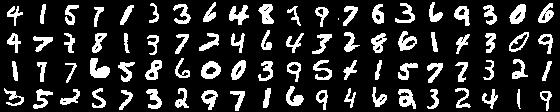
\includegraphics[scale=0.5]{images/mnist_dataset_example}
        \end{figure}
        \FloatBarrier
\end{enumerate}

\subsection{CIFAR Dataset}

\begin{enumerate}
  \item The CIFAR datasets are two datasets that contain a set of labelled $32x32$ color images. There are two
        versions of the dataset: one where the images are divided into 10 classes (CIFAR-10) and one where they are divided
        into 100 different classes (CIFAR-100). For this project, the CIFAR-100 dataset was used with a focus of the "coarse"
        labels provided (there are 20 coarse labels and 100 fine labels)
  \item These datasets are labelled subsets of the Tiny Images Dataset. The Tiny Images Dataset is a dataset of 80 million
        different $32x32$ images. The CIFAR datasets are comprised of a sampling of these images where the chosen images have
        been divided into classes and labelled.
  \item Within the context of this project, the CIFAR dataset was used as input to the Convolutional Neural Network as a more complex
        dataset than the MNIST dataset with real world (useful) classes that could be used in the identification process. A copy of the
        dataset was constructed where the images have been simplified by reducing their size to $28x28$ and converted to grayscale images.
        The images have also been whitened using PCA
        \FloatBarrier
        \begin{figure}
          \centering
          \begin{subfigure}{\textwidth}
            \centering
            \caption{Sample of original CIFAR dataset}
            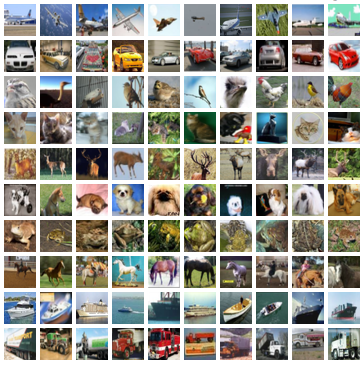
\includegraphics[scale=0.4]{images/cifar_dataset_example}
          \end{subfigure}
        \end{figure}
        \FloatBarrier
\end{enumerate}

\subsection{Custom Dataset}

\begin{enumerate}

\end{enumerate}

\section{Overview of Techniques}

This project involved the exploration of a number of techniques used to determine the features of an image. The technique that was settled
on and used for the attempted gathering of results was the Convolutional Neural Network. Other explored results were the use of Principal
Components Analysis on a set of images as well as simple MultiLayer Perceptrons and Logistic Regression. This report will go into detail on
the approach taken for testing each of these techniques as well as their results with respect to the goal of the project.

\subsection{Principal Components Analysis and Whitening}
  \subsubsection{Technique Overview}
  
  Principal Components Analysis (PCA) is a technique for converting a set of correlated variables into a set of linearly uncorrelated variables
  called Principal Components. The Principal Components are orthogonal to each other and starting with the first Principal Component, represent
  (in decreasing order) the largest possible variance. These Principal Components can be found by taking the eigendecomposition of the covariance
  matrix of a set of data. The Principal Components correspond to the eigenvectors of this decomposition.

  \subsubsection{Implementation}

  \subsubsection{Results and Analysis}





\section{Results and Further Work}

\section{Project Criterion Overview}

\end{document}
